\documentclass[conference, a4paper]{IEEEtran}

% used for flow charts
\usepackage{pgf}
\usepackage{tikz}
\usepackage{tikz-qtree}
\usepackage{reotex}

% package url is used when citing a website
\usepackage{url}

\usepackage{amssymb}
\usepackage{cite}
\usepackage[normalem]{ulem}
% for a smile-face character
\usepackage{wasysym}
% listing for codes
\usepackage{listings}

% positioning is used for below lef = of
\usetikzlibrary{shapes,arrows,automata,positioning}
% some tikz-styles on reo channels, not required in papers that have nothing to do with Reo

% FIXME finally no todos should exist in this draft
\usepackage[textsize=tiny]{todonotes}

% -------------------------------------- configurations -----------------------------------------
% declaration of environments
\newtheorem{theorem}{Theorem}
\newtheorem{definition}{Definition}
\newtheorem{example}{Example}

% personal characters
\newcommand{\rblock}[0]{\circleddash}
\newcommand{\rread}[0]{\smiley}
\newcommand{\rnoread}[0]{\frownie}


% --------------------------------------- information -------------------------------------------
\title{Active Learning from Blackbox to Timed Connectors}
\author{
\IEEEauthorblockN{Yi Li\IEEEauthorrefmark{1} and Meng Sun\IEEEauthorrefmark{1}}
\IEEEauthorblockA{
\IEEEauthorrefmark{1}Department of Informatics, School of Mathematical Sciences, Peking University,
Beijing, China\\
liyi\_math@pku.edu.cn, summeng@math.pku.edu.cn
}
}

\begin{document}
\maketitle
\begin{abstract}
  Coordination models and languages play a key role in formally specifying the communication and
  interaction among different components in large-scale distributed and concurrent systems. In this
  paper, we propose an active learning framework to extract timed connector models from black-box
  system implementation. 
  We first introduce parameterized mealy machine as an operational semantic
  model for channel-based coordination language Reo. Parameterized mealy machine serves as a bridge
  between Reo connectors and mealy machines. With the product operator, complex connectors can be
  constructed by joining basic channels and transformed into mealy machines. Moreover, we adapt L*,
  a well-known learning algorithm, to timed connectors (in the form of mealy machines). The new
  algorithm has shown its efficiency in multiple case studies. 
  Implementations of this framework is provided as a package in \texttt{Golang}.
\end{abstract}

\begin{IEEEkeywords}
  Active Learning, Coordination Languages, Formal Methods
\end{IEEEkeywords}

\section{Introduction}

In the past few years, researchers have been focusing on this area, and come up with a
series of impressive works. 
\todo{a list}
However, most of these works are based on models, instead of binaries. Then it comes a well-known
problem: \emph{how can we obtain these models?}

To solve this problem, many techniques in model constructing were proposed, for instance in
\cite{DBLP:journals/mt/Daelemans10, DBLP:journals/iandc/Angluin87, DBLP:conf/fase/RaffeltS06}.

% it seems that we need a graph to describe how we're doing this work
\todo{better graph}
% Define block styles
\tikzstyle{block} = [rectangle, draw, fill=blue!20, 
text width=4em, text centered, rounded corners, minimum height=3em]
\tikzstyle{line} = [draw, -latex']
\tikzstyle{cloud} = [draw, ellipse,fill=red!20, minimum height=2em, node distance = 2.5cm]

\begin{figure}[h]
  \centering
  \begin{tikzpicture}[node distance = 1.5cm, auto]
    % Place nodes
    \node [block] (reomodel) {REO Models};
    \node [cloud, left of=reomodel] (human) {Human};
    \node [block, below left = of reomodel] (tsamodel) {TSA};
    \node [block, below right = of reomodel] (mealymodel) {Mealy Machines};
    %\node [cloud, left = of tsamodel] (verification) {Verification};
    %\node [cloud, right = of mealymodel] (blackbox) {Blackbox};
    % Draw edges
    \path [line] (reomodel) -- (tsamodel);
    \path [line] (reomodel) -- (mealymodel);
    %\path [line] (tsamodel) -- (evaluate);
    \path [line] (mealymodel) -- (tsamodel);
    \path [line] (mealymodel) |-  (reomodel);
    %\path [line] (update) |- (tsamodel);
    %\path [line] (decide) -- node {no}(stop);
    %\path [line,dashed] (human) -- (reomodel);
  \end{tikzpicture}
  \caption{Our Idea}
  \label{fig:idea}
\end{figure}


In this paper, we presented an adapted active learning algorithm to extract timed Reo connectors
from binaries with no source code needed.

\section{Preliminaries}

\subsection{Reo Coordination Language}
\label{sec:reo}
Reo is a channel based exogenous coordination language proposed by F. Arbab. in
\cite{DBLP:journals/mscs/Arbab04}. A Reo model, also called \emph{connector}, provides the protocol
that formalizes the communication, synchronization and cooperation among the components which
communicate through the connector. Connectors can be defined with no knowledge of the components,
which makes Reo a powerful ``glue language'' in component-based
development\cite{DBLP:journals/sigsoft/Gill03}.

In Reo, complex connectors are made up of simpler ones, where the atomic connectors are called
\emph{channels}. Each channel has two \emph{channel ends}. There are two type of channel ends:
\emph{source} and \emph{sink}. Source channel ends accepts data into the channel, while sink
channels ends release them out of the channel. Channels are attached on component instances
or \emph{nodes}.



The behavior of some channels are informally described as follows. (Graphical representations
can be found in Figure \ref{fig:basic}).

\begin{itemize}
  \item [-] A \emph{Sync} channel accepts a data item from its source end iff. the data item can be
    dispensed to its sink end simultaneously.
  \item [-] A \emph{LossySync} channel is always prepared to accept data items. These items will be
    send to its sink end simutaneously if possible, otherwise they will be dropped.
  \item [-] A \emph{SyncDrain} channel has two source ends and no sink end. It can accept a data
    item through one of its source end iff. a data item is also available for it to simultaneously
    accept through the other end. Then both two data items will be lost.
  \item [-] 
\end{itemize}

\begin{figure}[h]
  \begin{center}
    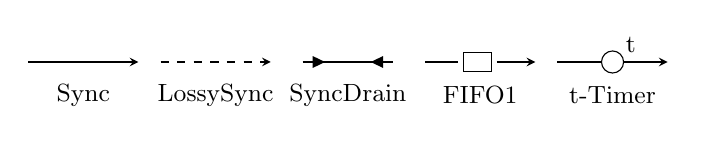
\begin{tikzpicture}[scale=1.4]

\tikzstyle{every node}=[font=\small]
\tikzstyle{label}=[draw=none]

\draw (0.5, -0.3) node[label] {Sync};
\draw (1.7, -0.3) node[label] {LossySync};
\draw (2.9, -0.3) node[label] {SyncDrain};
\draw (4.1, -0.3) node[label] {FIFO1};
\draw (5.3, -0.3) node[label] {t-Timer};

\sync{(0,0)}{(1,0)}{}
\lossysync{(1.2,0)}{(2.2,0)}{}
\syncdrain{(2.4,0)}{(3.4,0)}{}
\fifoe{(3.6,0)}{(4.6,0)}{}

\timer{(4.8,0)}{(5.8,0)}{node [above left] {t}}

\end{tikzpicture}

  \end{center}
  \caption{Basic Reo Channels}
  \label{fig:basic}
\end{figure}

\todo{do we need to remove this graph?}
\begin{figure}[h]
  \begin{center}
    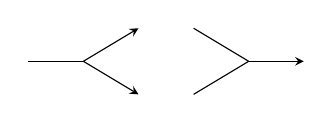
\begin{tikzpicture}[scale=1.4]

% replicator
\draw (0,0) -- (0.5,0);
\sync{(0.5,0)}{(1,0.3)}{}
\sync{(0.5,0)}{(1,-0.3)}{}

% replicator
\sync{(2,0)}{(2.5,0)}{}
\draw (1.5,0.3) -- (2,0);
\draw (1.5,-0.3) -- (2,0);

\end{tikzpicture}

  \end{center}
  \caption{Merger and Replicator}
  \label{fig:reoextend}
\end{figure}

\subsection{Mealy Machines}

As an extension of \emph{finite state machine}, Mealy machine was first proposed by George. H. Mealy
in \cite{George1955A}. Compared with other variants, Mealy machines are designed to model
reactive systems, where outputs are determined not only by its current state but also the current
inputs. Besides, Mealy machines are supposed to be \emph{input enabled}, which means that all
possible inputs should be acceptable in all states. In other words, if an input is invalid for some
state, we need to manually use an additional state to describe such exceptions.

As far as we can see, various forms of Mealy machines are defined in different works. In this paper,
we give the formal definition of Mealy machine following \cite{DBLP:conf/sfm/SteffenHM11}.

\todo{why we choose this version}

\begin{definition}[Mealy machine]
  A Mealy machine is a 6-tuple $(S, s_0, I, O, T, G)$ consisting of the following:
  \begin{itemize}
    \item[-] a finite set of states $S$
    \item[-] a start state (also called initial state) $s_0$ which is an element of $S$
    \item[-] a finite set called the input alphabet $I$
    \item[-] a finite set called the output alphabet $O$
    \item[-] a transition function $\delta : S \times I \rightarrow S$ mapping pairs of a
      state and an input symbol to the corresponding next state.
    \item[-] an output function $\lambda : S \times I \rightarrow O$ mapping pairs
      of a state and an input symbol to the corresponding output symbol.
  \end{itemize}
\end{definition}

\subsection{Active Learning}

\section{Timed Connectors as Mealy Machines}

\subsection{External Behavior of Reo Connectors}
So far as we can tell, most
works\cite{DBLP:conf/fase/RaffeltS06, DBLP:journals/corr/ChenHLLTWW15} on automata learning are not
capable of infinite models. \todo{reason?} Considering the semantics defined in section
\ref{sec:reo}, it's apparent that every finite connector has a corresponding constraint
automata, and the automata is also finite. Unfortunately, when checking the further definition of
Reo connectors' input, we find that it's not the case.

\todo{an example as graph}

\begin{figure}[h]
  \caption{Infinite States in a Reo Model}
  \label{fig:reoinfinite}
\end{figure}

While focusing on behavior of connectors, Reo doesn't give detail depiction on behavior of
components. As shown in \figurename \ref{fig:reoinfinite}, connectors are able to reject any datum
if they are not ready. But what will happen outside the connector, if the datum is rejected? This
question deserves careful consideration if we are taking an external view.

\subsection{Time Domain}
Time is involved in several extension version of Reo. For example, Timed
Reo\cite{DBLP:conf/sefm/ArbabBBR04}, Hybrid Reo\cite{DBLP:conf/icfem/ChenSS14}, etc.
Generally, these models are designed to handle real-time behavior where time is defined in
$\mathbb{R}$. However, we also found a lot of works where authors use rational time to make things
easier.

In this paper, we choose the rational number field $\mathbb{Q}$ as our time domain, which simplifies
discretization of timed behaviors greatly.

As presented in section \ref{sec:reo}, all real-time behavior in timed Reo comes with the
\emph{t-timer} channels, and the number of these channels are apparently finite. We use
$t_i\in\mathbb{Q}$ to denote the delays of these timer channels, and now we can define a precision
function $prec$.
\[
prec(t_1,\cdots,t_n) = \max_T\{\forall t_i.\exists n_i\in\mathbb{N}.t_i=n_i\cdot T\}
\]
It's easy to prove that such a $T$ is always existing.

In real systems, the concept \emph{time precision} is widely used with the name ``clock-period''.
Most of the time, we know the clock-cycle of some hardware components, even without any idea of its
structure. With such precision $T$ given, it's reasonable to assume that all $t$-timers are actually
$nT$-timers. In following sections, we'll use $n$-timers instead.

Besides, we're going to add a ``T'' action in mealy machines. It indicates that a transition
will take a time unit to finish, and all outputs would come out after that.

\subsection{Parameterized Mealy Machine}
We present a model named \emph{parameterized mealy machine} to represent timed connectors
(hereinafter referred to as PMM). 

This model is supposed to behave as a middle representation. Connectors are defined as parameterized
mealy machines, and composed via its production operator. Then original mealy-machine model will be
taken as semantics of PMM model.

\begin{definition}[Parameterized Mealy Machine]
  A \emph{Parameterized Mealy Machine} is defined as a function $\mathcal{PM}(\Sigma)=\langle
  S(\Sigma), s_0, I, O, \delta(\Sigma), \lambda(\Sigma)\rangle$ that maps an
  alphabet to its corresponding Mealy Machine. 
  \begin{itemize}
    \item[-] $\Sigma$ is a \emph{finite} datum alphabet (hereinafter referred to as an alphabet)
    \item[-] $S$ is a function that maps an alphabet to a \emph{finite} set of
      states. We use $S(\Sigma)$ to denote the state set.
    \item[-] $I$ is a finite set of source-ends.
    \item[-] $O$ is a finite set of sink-ends.
    \item[-] $s_0$ is the initial state. It satisfies $\forall \Sigma,s_0\in S(\Sigma)$
    \item[-] $\delta$ maps a \emph{finite} datum alphabet to an \emph{output function}. We use
      $\delta(\Sigma):S(\Sigma)\times Input(\Sigma,I)\rightarrow Output(\Sigma, O)$ to denote the output function.
    \item[-] $\lambda$ maps an alphabet to a \emph{transition function}. We use
      $\lambda(\Sigma):S(\Sigma)\times Input(\Sigma,I)\rightarrow S(\Sigma)$ to denote the transiton
      function.
  \end{itemize}
\end{definition}

In the definition above, \emph{Input} and \emph{Output} are used to generate input actions and output actions by the corresponding alphabets and ends.
\todo{How to say?}
\[
Input(\Sigma,I)=\{\}\cup\{T\}
\]
where we use $T$ to denote the time action.
\[
Output(\Sigma,I)=\{\}
\]

Now we can use Parameterized Mealy Machines to define a new semantics to Reo.
\begin{example}[PMM Semantics of FIFO channel $PM_{FIFO}$]
  \label{example:pmmfifo}
  The semantics of FIFO channel with source end $A$ and sink end $B$ can be defined as follows.
  \begin{itemize}
    \item[-] $S(\Sigma)=\{q_0\}\cup\{q_d|d\in\Sigma\}$
    \item[-] $I=\{A\}$
    \item[-] $O=\{B\}$
    \item[-] $s_0=q_0$
    \item[-] output function
      \begin{displaymath}
        \delta(\Sigma)(s,i)=\left\{
        \begin{array}[h]{ll}
          (B:\bot) & s=q_0\land i=(A:\_,B:\rnoread) \\
          (B:d) & s=q_0\land i=(A:d,B:\rread)\\
          \rblock & s=q_0\land i=(A:\bot,B:\rread) \\
          (B:d) & s=q_d\land i=(A:\_,B:\rread)\\
          \rblock & s=q_d\land i=(A:d,B:\rnoread) \\
          (B:\bot) & s=q_d\land i=(A:\_,B:\rnoread) \\     
        \end{array}
        \right.
      \end{displaymath}
    \item[-] transition function
      \begin{displaymath}
        \lambda(\Sigma)(s,i)=\left\{
        \begin{array}[h]{ll}
          q_d & s=q_0\land i=(A:d,B:\rnoread) \\
          q_d & s=q_{d'}\land i=(A:d,B:\rread) \\
          q_0 & otherwise \\
        \end{array}
        \right.
      \end{displaymath}
  \end{itemize}
\end{example}

Besides, the concrete mealy machine (where $\Sigma=\{a\}$) is shown in Figure \ref{fig:pmmfifo}.
\begin{figure}[h]
  \begin{center}
    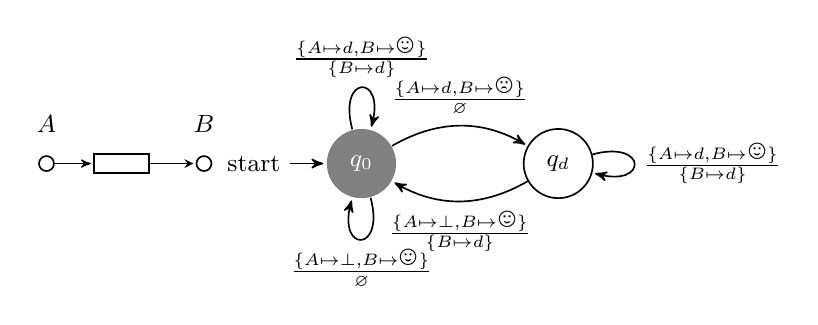
\begin{tikzpicture}[->,>=stealth',shorten >=1pt,auto,node distance=1.6cm,
  semithick]
  \tikzstyle{every node}=[font=\small]
  \ionode{(P-A)}{(-4,0)}{(-4,0.5) node {$A$}}
  \ionode{(P-B)}{(-2,0)}{(-2, 0.5) node {$B$}}
  
  \fifoe{(P-A)}{(P-B)}{}

  \tikzstyle{every state}=[fill=white,text=black,font=\small]
  \tikzstyle{init}=[fill=gray,draw=none,text=white]

  \node[initial,state,init] (Q0)                     {$q_{0}$};
  \node[state]         (QA)  [right = of Q0]    {$q_{d}$};

  \path
  (Q0)
  edge  [bend left]     node {$\frac{\{A\mapsto d, B\mapsto \rnoread\}}{\varnothing}$} (QA)
  edge  [loop below]    node {$\frac{\{A\mapsto \bot, B\mapsto \rread\}}{\varnothing}$} (QA)
  edge  [loop above]    node {$\frac{\{A\mapsto d, B\mapsto \rread\}}{\{B\mapsto d\}}$} (QA)
  (QA)
  edge  [bend left]     node {$\frac{\{A\mapsto \bot,B\mapsto \rread\}}{\{B\mapsto d\}}$} (Q0)
  edge  [loop right]    node {$\frac{\{A\mapsto d,B\mapsto \rread\}}{\{B\mapsto d\}}$} (QA)
  ;
\end{tikzpicture}


  \end{center}
  \caption{PMM-based Semantics of FIFO, where $\Sigma=\{a\}$}
  \label{fig:pmmfifo}
\end{figure}

Similarly, we can use parameterized mealy machines to define the semantics of other basic timed Reo
channels. Now we're going to show how to compose these channels into complicated connectors.

\begin{definition}[Production of Parameterized Mealy Machines]
  Now we're going to define the production operator \emph{prod} of two parameterized mealy machines as,
  \[
  prod(PM_1,PM_2)=PM_3
  \]
  as follows. Here we assume that $PM_2.O\cap PM_1.I=\varnothing$
  \begin{itemize}
  	\item[-] $\forall\Sigma, PM_3.S(\Sigma)=PM_1.S(\Sigma)\times PM_2.S(\Sigma)$
    \item[-] $PM_3.I=PM_1.I\cup PM_2.I-PM_1.O$
    \item[-] $PM_3.O=PM_1.O\cup PM_2.O-PM_2.I$
    \item[-] $PM_3.s_0=(PM_1.s_0, PM_2.s_0)$
    \item[-] $\forall\Sigma, PM_3.\delta(\Sigma)((s_1,s_2), i)=$
      \begin{displaymath}
        \left\{
        \begin{array}[h]{ll}
          (Out_1 + Out_2)|_{PM_3.O} & \rblock\land Out_2\neq\rblock \\
          \rblock & otherwise \\
        \end{array}
        \right.
      \end{displaymath}
      where we have
      \begin{itemize}
        \item[*] $In_1 = i|_{PM_1.I}$
        \item[*] $Out_1 = PM_1.\delta(\Sigma)(s_1,In_1)$
        \item[*] $In_2 = (Out_1 + i)|_{PM_2.I}$
        \item[*] $Out_2 = PM_2.\delta(\Sigma)(s_2,In_2)$
      \end{itemize}
    \item[-] $\forall\Sigma, PM_3.\lambda(\Sigma)((s_1,s_2),i)=(s_1',s_2')$
      where we have
      \begin{itemize}
        \item[*] $s_1' = PM_1.\lambda(\Sigma)(s_1,In_1)$
        \item[*] $s_2' = PM_2.\lambda(\Sigma)(s_2,In_2)$
      \end{itemize}
  \end{itemize}
\end{definition}

\todo{example of production, maybe fifo+timer}

\section{From Blackbox to Timed Connectors}

\subsection{Observation Table}

\subsection{Closeness}

\subsection{Counter-Examples}
Generally, equivalence query has been proved impossible in blackbox
models\cite{DBLP:journals/iandc/Angluin87}. However, in this
section, we're showing that in certain circumstances, equivalence query can be implemented with
no approximation.

Equivalence queries are used to search for counter-examples. But what makes counter-examples even
existing? In Reo models, we believe that \emph{FIFO} channels and \emph{Timer} channels are to
blame. Here we present a brief example. To make things eaiser, we have only untimed Reo here.

\begin{figure}[h]
  \begin{center}
    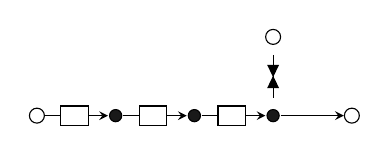
\begin{tikzpicture}

  \ionode{(P-A)}{(0,0)}{}
  \ionode{(P-B)}{(3,1)}{}
  \mixednode{(P-M1)}{(1,0)}{}
  \mixednode{(P-M2)}{(2,0)}{}
  \mixednode{(P-M3)}{(3,0)}{}
  \ionode{(P-C)}{(4,0)}{}

  \fifoe{(P-A)}{(P-M1)}{}
  \fifoe{(P-M1)}{(P-M2)}{}
  \fifoe{(P-M2)}{(P-M3)}{}
  \syncdrain{(P-B)}{(P-M3)}{}
  \sync{(P-M3)}{(P-C)}{}

\end{tikzpicture}

  \end{center}
  \caption{A Switching Connector $S$ with Three Buffers}
  \label{fig:buf3}
\end{figure}

A \emph{Switching} connector in \figurename \ref{fig:buf3} has two source-ends $A,B$ and one
sink-end $C$. In a nutshell, datum come from $A$ and be stored temporarily in buffers. These datum
will never flow out until signals come to $B$. With the Mealy-Machine semantics given, the semantics
of \emph{Switching} connectors can be defined as following \figurename \ref{fig:buf3semantics}.

\begin{figure}[h]
  \begin{center}
    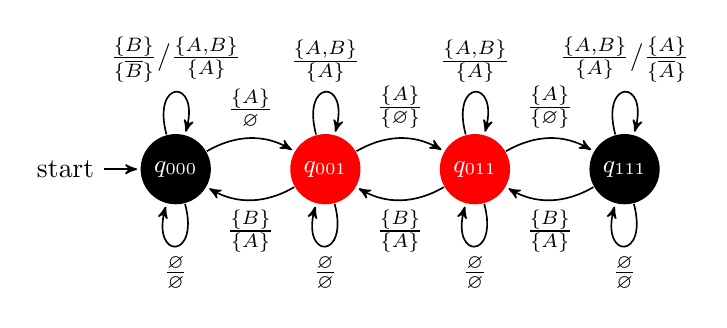
\begin{tikzpicture}[->,>=stealth',shorten >=1pt,auto,node distance=1.9cm,
                    semithick]
  \tikzstyle{every state}=[fill=black,draw=none,text=white,font=\small]
  \tikzstyle{red}=[fill=red]

  \node[initial,state] (Q000)                    {$q_{000}$};
  \node[state,red]         (Q001) [right of=Q000] {$q_{001}$};
  \node[state,red]         (Q011) [right of=Q001] {$q_{011}$};
  \node[state]         (Q111) [right of=Q011] {$q_{111}$};

  \path (Q000) edge  [bend left]   node {$\frac{\{A\}}{\varnothing}$} (Q001)
               edge  [loop below]  node {$\frac{\varnothing}{\varnothing}$} (Q001)
               edge  [loop above]  node {$
                                     \frac{\{B\}}{\{\overline{B}\}}/
                                     \frac{\{A,B\}}{\{A\}}
                                   $} (Q000)
        (Q001) edge  [bend left]   node {$\frac{\{B\}}{\{A\}}$} (Q000)
               edge  [loop below]  node {$\frac{\varnothing}{\varnothing}$} (Q001)
               edge  [loop above]  node {$
                                     \frac{\{A,B\}}{\{A\}}
                                   $} (Q001)
               edge  [bend left]   node {$\frac{\{A\}}{\{\varnothing\}}$} (Q011)
        (Q011) edge  [bend left]   node {$\frac{\{B\}}{\{A\}}$} (Q001)
               edge  [loop below]  node {$\frac{\varnothing}{\varnothing}$} (Q011)
               edge  [loop above]  node {$
                                     \frac{\{A,B\}}{\{A\}}
                                   $} (Q011)
               edge  [bend left]   node {$\frac{\{A\}}{\{\varnothing\}}$} (Q111)
        (Q111) edge  [bend left]   node {$\frac{\{B\}}{\{A\}}$} (Q011)
               edge  [loop below]  node {$\frac{\varnothing}{\varnothing}$} (Q111)
               edge  [loop above]  node {$
                                     \frac{\{A,B\}}{\{A\}}/
                                     \frac{\{A\}}{\{\overline{A}\}}
                                   $} (Q111)
        %(B) edge [loop above] node {1,1,L} (B)
            %edge              node {0,1,L} (C)
        %(C) edge              node {0,1,L} (D)
            %edge [bend left]  node {1,0,R} (E)
        %(D) edge [loop below] node {1,1,R} (D)
            %edge              node {0,1,R} (A)
  ;
\end{tikzpicture}


  \end{center}
  \caption{\emph{Gate} as Mealy Machine $\mathcal{M}(S)$}
  \label{fig:buf3semantics}
\end{figure}

According to the production of Mealy-Machines, 8 different states should be found in
$\mathcal{M}(S)$. We use $q_{abc}$ to denote them. $q_{001}$ indicates that the last buffer is
filled and others are empty, and $q_{111}$ means that there are no space in any buffer. It's
obvious that some states like $q_{100}$ is unreachable.

We say if two states are \emph{similiar} iff. they have the same output signature.

\begin{theorem}[Bound of Counter-Example]
  \label{the:cebound} Assume that an observation table has already been closed with maximum
  query length \todo{find a better phrase?} $l$. An counter-example of length $l+2$ would be
  found iff. there're possible counter-examples.
\end{theorem}
\begin{IEEEproof}
  Sketch of this proof are shown in several points:
  \begin{enumerate}
    \item Hypothesises are subgraphs of the semantics graph.
    \item Inputs on reverse edges are complementary.
    \item 
  \end{enumerate}
\end{IEEEproof}

\section{Experiments}
Both \emph{Reo Coordination Models} and \emph{Adapted L* Algorithm} are implemented in
Golang\cite{golang}.

Golang (or Google Go) is a rising programming language started by Google Inc. The language is widely
known for its elegant design and impressive efficiency. Moreover, the concurrency model of Golang
comes from CSP\cite{DBLP:books/ph/Hoare85}. As a channel-based model, CSP shares a similar idea with
Reo and makes our implementation much more natural.

We have programmed Reo channels as a new package in Golang. The package is well-written for not only
formal verification but also practical use.

All the following experiments are coded under Golang \emph{1.2.1} and executed on a laptop with 8GB
of RAM and a Core i7-3630 CPU. The source code is available at
\url{https://github.com/liyi-david/reo-learn}.

\subsection{Case Studies}
 
\subsection{Performance Optimization}
As a well-known learning algorithm, L* has proved its efficiency in models without time.
However, when dealing with timed connectors, the algorithm failed to meet our expectation.

\begin{table}[h]
  \renewcommand{\arraystretch}{1.3}
  \caption{Time-Cost Analysis}
  \label{tabel:timecost}
  \centering
  \begin{tabular}{l||rrr}
    \hline
    & FIFO & Alternator & Gate \\
    \hline\hline
    Membership Query(s) & 41.571 & 126.468 & 169.161 \\
    Hypothesis Query(s) & 0.001 & 0.003 & 0.004 \\
    Total Time(s) & 41.715 & 165.114 & 247.098\\
    Membership Query(\%) & 99.6 & 76.6 & 68.5\\
    \hline
  \end{tabular}
\end{table}

As shown in Table \ref{tabel:timecost}, time consumption mainly comes from membership queries.
Since time is involved in our model, it's inevitably that simulation takes time to behave normally.
Even worse, since our models are treated as blackbox. With no access to inner behaviour of the
connectors, it's almost impossible to accelerate the simulation process.

Fortunately, there are still other optimization solutions. After reviewing our algorithm, we found
that simulations on similar sequences were invoked frequently:

\begin{itemize}
  \item When constructing \emph{Obs} tables, there are lots of redundant calls to membership
    queries. For example, a sequence with prefix 'aa' and suffix 'b' is exactly same as another one
    with prefix 'a' and suffix 'ab'.
  \item Simulation on mealy machines can provide multi-step output. Consequently, if we has
    simulated an 'abc' sequence, there's no reason to perform simulation on an 'ab' sequence.
\end{itemize}

If previous simulation results are stored in a well-maintained cache, the time-cost in
simulation process could be reduced signficiantly. In this work, we use a multiway tree to buffer
these results. A brief example of such trees can be found in Figure \ref{fig:multiway}.

\todo{the graph need further details}
\begin{example}[Multiway-Tree Cache]
  \label{example:tree}
  Considering the FIFO channel presented in Example \ref{example:pmmfifo}. 
  \begin{figure}[h]
    \begin{center}
      \begin{tikzpicture}

\tikzset{grow'=right, level distance=42pt}
\tikzset{execute at begin node=\strut}
\tikzset{every tree node/.style={anchor=base west}}

\Tree [.$q_0$ [.$q_0$ [.$q_0$ ... ] [.$q_a$ ] ... ] [.$q_a$ ... ] ]
\end{tikzpicture}

    \end{center}
    \caption{Multiway-Tree Cache}
    \label{fig:multiway}
  \end{figure}
  Note that in this figure, only the edge information is stored. States like $q_0,q_a$ are written
  here only to make it clear.
\end{example}

\begin{table}[h]
  \renewcommand{\arraystretch}{1.3}
  \caption{Reduction of Membership Queries}
  \label{tabel:cacheoptimization}
  \centering
  \begin{tabular}{l||rrr}
    \hline
    & FIFO & Alternator & Gate \\
    \hline\hline
    Original Algorithm & 93 & 880 & 1034 \\
    Cached Algorithm & 90 & 725 & 707 \\
    Reduction Rate & 3.2\% & 21.4\% & 31.6\% \\
    \hline
  \end{tabular}
\end{table}

With cache applied, we have made a good reduction on the calls of membership queries. The results
can be found in Table \ref{tabel:cacheoptimization}.

\subsection{An Example of the Reo Package}
As mentioned above, our implementation in \texttt{Golang} is well-prepared not only for academic use
but also for practical concurrent programming.

\todo{modify the listings package}
\begin{lstlisting}
int main(int argc, char ** argv)
{
  printf(``Hello world!n'');
  return 0;
}
\end{lstlisting}

\section{Conclusion and Future Work}



\bibliographystyle{abbrv}
\bibliography{bib}

% FIXME remove this
\listoftodos

\end{document}
